\section{Group -- Humidifiers and Dehumidifiers}\label{group-humidifiers-and-dehumidifiers}

\subsection{Humidifier:Steam:Electric}\label{humidifiersteamelectric}

The electric steam humidifier is a component that represents an electrically heated, self contained steam humidifier. The component uses electrical energy to convert ordinary tap water to steam which it then injects into the supply air stream by means of a blower fan. The actual unit might be an electrode-type humidifier or a resistance-type humidifier.

The humidifier model includes local control of the humidifier unit to meet a humidity ratio setpoint on its air outlet node. A set point manager is needed to put a setpoint on the exit node but no other local controllers are needed. The humidifier will add moisture to meet the humidity ratio setpoint.

\subsubsection{Inputs}\label{inputs-023}

\paragraph{Field: Name}\label{field-name-022}

A unique user assigned name for a particular humidifier unit. Any reference to this unit by another object will use this name.

\paragraph{Field: Availability Schedule Name}\label{field-availability-schedule-name-010}

The name of the schedule (ref: Schedule) that denotes whether the unit can run during a given time period. A schedule value of 0 indicates that the unit is off for that time period. A schedule value greater than 0 indicates that the unit can operate during the time period. If this field is blank, the schedule has values of 1 for all time periods.

\paragraph{Field: Rated Capacity}\label{field-rated-capacity-000}

The nominal full output water addition rate of the unit in m\(^{3}\)/sec of water at 5.05 C. This field is autosizable.

\paragraph{Field: Rated Power}\label{field-rated-power-000}

The nominal full output power consumption of the unit in watts, exclusive of the blower fan power consumption and any standby power. This field can be autosized. When it is autosized, its calculated from the rated capacity in kg/s and the enthalpy rise in J/kg of the feed water from the a reference temperature of liquid water at 20 °C to a saturated steam at 100 °C.

\paragraph{Field: Rated Fan Power}\label{field-rated-fan-power}

The nominal full output power consumption of the blower fan in watts.

\paragraph{Field: Standby Power}\label{field-standby-power-000}

The standby power consumption in watts. This amount of power will be consumed whenever the unit is available (as defined by the availability schedule).

\paragraph{Field: Air Inlet Node Name}\label{field-air-inlet-node-name-004}

The name of the HVAC system node from which the unit draws inlet air.

\paragraph{Field: Air Outlet Node Name}\label{field-air-outlet-node-name-004}

The name of the HVAC system node to which the unit sends its outlet air.

\paragraph{Field: Water Storage Tank Name}\label{field-water-storage-tank-name}

This field is optional. If left blank or omitted, then the humidifier obtains its water directly from the mains water. If the name of a Water Storage Tank is specified, then the humidifier will try to obtain its water from that tank. If the tank can t provide all the water then the rest will be drawn from the mains and the humidifier will still operate.

An IDF example:

\begin{lstlisting}

Humidifier:Steam:Electric,
  Humidifier 1,                   !- Name
  FanAndCoilAvailSched,   !- Availability Schedule Name
  0.00000379,                       !- Rated Capacity {m3/s}
  10200.,                               !- Rated Power {W}
  27.,                                     !- Rated Fan Power {W}
  2.,                                       !- Standby Power {W}
  Cooling Coil Air Outlet Node, !- Air Inlet Node Name
  Air Loop Outlet Node;   !- Air Outlet Node Name
\end{lstlisting}

\subsubsection{Outputs}\label{outputs-016}

\begin{itemize}
\item
  HVAC,Average,Humidifier Water Volume Flow Rate {[}m3/s{]}
\item
  HVAC,Sum,Humidifier Water Volume{[}m3{]}
\item
  HVAC,Average,Humidifier Electricity Rate {[}W{]}
\item
  HVAC,Sum,Humidifier Electricity Energy {[}J{]}
\item
  Zone,Meter,Humidifier:Water {[}m3{]}
\item
  Zone,Meter,Humidifier:Electricity {[}J{]}
\item
  HVAC,Average,Humidifier Storage Tank Water Volume Flow Rate {[}m3/s{]}
\item
  HVAC,Sum,Humidifier Storage Tank Water Volume {[}m3{]}
\item
  HVAC,Average,Humidifier Starved Storage Tank Water Volume Flow Rate {[}m3/s{]}
\item
  HVAC,Sum,Humidifier Starved Storage Tank Water Volume {[}m3{]}
\item
  Zone,Meter,Humidifier:MainsWater {[}m3{]}
\item
  HVAC,Sum,Humidifier Mains Water Volume {[}m3{]}
\end{itemize}

\paragraph{Humidifier Water Volume Flow Rate {[}m3/s{]}}\label{humidifier-water-volume-flow-rate-m3s}

This field reports the water consumption rate of the steam humidifier in cubic meters of water per second.

\paragraph{Humidifier Water Volume{[}m3{]}}\label{humidifier-water-volumem3}

This output is the cubic meters of water consumed by the steam humidifier over the timestep being reported.

\paragraph{Humidifier Electricity Rate {[}W{]}}\label{humidifier-electric-powerw}

This output is the electricity consumption rate in Watts of the steam humidifier.

\paragraph{Humidifier Electricity Energy {[}J{]}}\label{humidifier-electric-energy-j}

This is the electricity consumption in Joules of the steam humidifier over the timestep being reported.

\paragraph{Humidifier:Water {[}m3{]}}\label{humidifierwater-m3}

This meter output contains the sum of the water consumed (in cubic neters of water during the report timestep) by all the steam humidifiers at the HVAC level in the simulation.

\paragraph{Humidifier:Electricity {[}J{]}}\label{humidifierelectricity-j}

This meter output contains the sum of the electricity consumed (in Joules during the report timestep) by all the steam humidifiers at the HVAC level in the simulation.

\paragraph{Humidifier Storage Tank Water Volume Flow Rate {[}m3/s{]}}\label{humidifier-storage-tank-water-volume-flow-rate-m3s}

\paragraph{Humidifier Storage Tank Water Volume {[}m3{]}}\label{humidifier-storage-tank-water-volume-m3}

These outputs contain the rate and volume of water obtained from water storage tank. These are only present if the humidifier is connected to a Water Storage Tank for its water supply.

\paragraph{Humidifier Starved Storage Tank Water Volume Flow Rate {[}m3/s{]}}\label{humidifier-starved-storage-tank-water-volume-flow-rate-m3s}

\paragraph{Humidifier Starved Storage Tank Water Volume {[}m3{]}}\label{humidifier-starved-storage-tank-water-volume-m3}

These outputs contain the rate and volume of water that could not be obtained from the water storage tank. The component will still operate as if it did get all the water with the balance obtained directly from the mains

\paragraph{Humidifier Mains Water Volume {[}m3{]}}\label{humidifier-mains-water-volume-m3}

This output contains the volume of water obtained from the mains.

\subsection{Humidifier:Steam:Gas}\label{humidifiersteamgas}

The gas fired steam humidifier is a component that represents a gas fired self-contained steam humidifier. The component uses gas fired energy to convert ordinary tap water to steam which it then blows or injects into the supply air stream. Blower fan may not be required depending on how the dry steam is delivered into the supply air stream. The humidifier model includes local control of the humidifier unit to meet a humidity ratio setpoint on its air outlet node of the unit. A humidity set point manager is needed to put a setpoint on the outlet node but no other local controllers are needed. The humidifier either blows or injects dry steam to meet the humidity ratio setpoint requirement. If the Rated Gas Use Rate input field is not autosized, the thermal efficiency input specified will be ignored and overridden by a thermal efficiency value determined from user specified Rated Gas Use Rate, rated capacity (m3/s) and design conditions for sizing calculation.

\subsubsection{Inputs}\label{inputs-1-021}

\paragraph{Field: Name}\label{field-name-1-020}

A unique user assigned name for a particular humidifier unit. Any reference to this unit by another object will use this name.

\paragraph{Field: Availability Schedule Name}\label{field-availability-schedule-name-1-008}

The name of the schedule (ref: Schedule) that denotes whether the unit can run during a given time period. A schedule value of 0 indicates that the unit is off for that time period. A schedule value greater than 0 indicates that the unit can operate during the time period. If this field is blank, the schedule has values of 1 for all time periods.

\paragraph{Field: Rated Capacity}\label{field-rated-capacity-1}

The nominal full capacity water addition rate in m3/s of water at 5.05 C.

\paragraph{Field: Rated Gas Use Rate \{W\}}\label{field-rated-gas-use-rate-w}

The nominal gas use rate in Watts. This input field can be autosized. When this input field is autosized, it is calculated from the rated capacity in kg/s, the enthalpy rise in J/kg of the feed water from a reference temperature of liquid water at 20 °C to a saturated steam at 100 °C and user specified thermal efficiency. If this input field is hardsized and the Inlet Water Temperature Option input field is selected as FixedInletWaterTemperature, then the thermal efficiency input field will not be used in the calculation or else if the Inlet Water Temperature Option input selected is VariableInletWaterTemperature, then the user specified thermal efficiency value will be overridden using internally calculated efficiency from the capacity, rated gas use rate and design condition.

\paragraph{Field: Thermal Efficiency}\label{field-thermal-efficiency}

The thermal efficiency of the gas fired humidifier. The thermal efficiency is based on the higher heating value of the fuel. The default value is 0.8. If Rated Gas Use Rate in the field above is not autosized and the Inlet Water Temperature Option input field selected is FixedInletWaterTemperature, then the thermal efficiency specified will be ignored in the calculation, or else if the Inlet Water Temperature Option input field is specified as VariableInletWaterTemperature, then the user specified thermal efficiency value will be overridden using internally calculated matching the capacity, rated gas use rate specified and design condition defined for sizing calculation.

\paragraph{Field: Thermal Efficiency Modifier Curve Name}\label{field-thermal-efficiency-modifier-curve-name}

This is thermal efficiency modifier curve name of unit. This curve is normalized, i.e., the curve output value at rated condition is 1.0. If this input field is blank, then constant efficiency value specified in the input field above will be used. Allowed thermal efficiency modifier curve types are linear, quadratic, or cubic. These curves are solely a function of part load ratio.

\paragraph{Field: Rated Fan Power}\label{field-rated-fan-power-1}

The nominal full capacity electric power input to the blower fan in Watts. If no blower fan is required to inject the dry steam to the supply air stream, then this input field is set to zero.

\paragraph{Field: Auxiliary Electric Power}\label{field-auxiliary-electric-power}

The auxiliary electric power input in watts. This amount of power will be consumed whenever the unit is available (as defined by the availability schedule). This electric power is used for control purpose only.

\paragraph{Field: Air Inlet Node Name}\label{field-air-inlet-node-name-1-004}

The name of the HVAC system node from which the unit draws inlet air.

\paragraph{Field: Air Outlet Node Name}\label{field-air-outlet-node-name-1-003}

The name of the HVAC system node to which the unit sends its outlet air.

\paragraph{Field: Water Storage Tank Name}\label{field-water-storage-tank-name-1}

This field is optional. If left blank or omitted, then the humidifier obtains its water directly from the mains water. If the name of a Water Storage Tank is specified, then the humidifier will try to obtain its water from that tank. If the tank can t provide all the water then the rest will be drawn from the mains and the humidifier will still operate.

\paragraph{Field: Inlet Water Temperature Option}\label{field-inlet-water-temperature-option}

This field is a key/choice field that tells which humidifier water inlet temperature to use: fixed inlet temperature or variable water inlet temperature that depends on the source. Currently allowed water sources are main water or water storage tank in water use objects. The key/choice are: FixedInletWaterTemperature, with this choice, the gas fired humidifier will use a fixed 20C water inlet temperature. VariableInletWaterTemperature, with this choice, the gas fired humidifier will use water inlet temperature that depends on the source temperature. If a water use storage tank name is specified, then the gas humidifier water inlet temperature will be the storage water temperature, or else it uses water main temperature. The default main water temperature is 10 °C. If left blank or omitted, then the humidifier assumes fixed inlet water temperature of 20 °C.

An IDF example:

\begin{lstlisting}

Humidifier:Steam:Gas,
  Main Gas Humidifier,!- Name
  ALWAYS_ON,          !- Availability Schedule Name
  4.00E-5,            !- Rated Capacity {m3/s}
  104000,             !- Rated Gas Use Rate {W}
  1.0,                !- Thermal Efficiency {-}
  ,                   !- Thermal Efficiency Modifier Curve Name
  0,                  !- Rated Fan Power {W}
  0,                  !- Auxiliary Electric Power {W}
  Mixed Air Node 1,   !- Air Inlet Node Name
  Main Humidifier Outlet Node,  !- Air Outlet Node Name
  ;                   !- Water Storage Tank Name
\end{lstlisting}

Steam Gas Humidifier Outputs

\begin{itemize}
\tightlist
\item
  HVAC,Average,Humidifier Water Volume Flow Rate {[}m3/s{]}
\item
  HVAC,Sum,Humidifier Water Volume{[}m3{]}
\item
  HVAC,Average,Humidifier NaturalGas Use Rate{[}W{]}
\item
  HVAC,Sum,Humidifier NaturalGas Use Energy {[}J{]}
 \item
  HVAC,Average,Humidifier NaturalGas Use Thermal Efficiency {[}{]}
\item
  HVAC,Average,Humidifier Auxiliary Electricity Rate {[}W{]}
\item
  HVAC,Sum,Humidifier Auxiliary Electricity Energy {[}J{]}
\item
  HVAC,Meter,Humidifier:Water {[}m3{]}
\item
  HVAC,Meter,Humidifier:NaturalGas {[}J{]}
\item
  HVAC,Meter,Humidifier:Electricity {[}J{]}
\item
  HVAC,Average,Humidifier Storage Tank Water Volume Flow Rate {[}m3/s{]}
\item
  HVAC,Sum,Humidifier Storage Tank Water Volume {[}m3{]}
\item
  HVAC,Average,Humidifier Starved Storage Tank Water Volume Flow Rate {[}m3/s{]}
\item
  HVAC,Sum,Humidifier Starved Storage Tank Water Volume {[}m3{]}
\item
  Zone,Meter,Humidifier:MainsWater {[}m3{]}
\item
  HVAC,Sum,Humidifier Mains Water Volume {[}m3{]}
\end{itemize}

\paragraph{Humidifier Water Volume Flow Rate {[}m3/s{]}}\label{humidifier-water-volume-flow-rate-m3s-1}

This field reports the water consumption rate of the steam humidifier in cubic meters of water per second.

\paragraph{Humidifier Water Volume {[}m3{]}}\label{humidifier-water-volume-m3}

This output is the cubic meters of water consumed by the steam humidifier over the timestep being reported.

\paragraph{Humidifier NaturalGas Use Rate {[}W{]}}\label{humidifier-naturalgas-use-rate-w}

This output is the natural gas use rate of the natural gas fired steam humidifier in Watts.

\paragraph{Humidifier NaturalGas Use Energy {[}J{]}}\label{humidifier-naturalgas-use-energy-j}

This output is the natural gas consumption of the natural gas fired steam humidifier in Joules.

\paragraph{Humidifier NaturalGas Use Thermal Efficiency {[}{]}}\label{humidifier-naturalgas-use-thermal-efficiency-j}

This output is the thermal efficiency of the natural gas consumed by the natural gas fired steam humidifier.

\paragraph{Humidifier Auxiliary Electricity Rate {[}W{]}}\label{humidifier-auxiliary-electric-power-w}

This output is the auxiliary electricity consumption rate in Watts of the gas fired steam humidifier. This is the auxiliary electric power input to the blower fan and control unit.

\paragraph{Humidifier Auxiliary Electricity Energy {[}J{]}}\label{humidifier-auxiliary-electric-energy-j}

This is the auxiliary electricity consumption in Joules of the gas fired steam humidifier over the timestep being reported. This is the auxiliary electric energy consumed by the blower fan and control unit. This auxiliary electric energy is reported meter output Humidifier:Electricity.

\paragraph{Humidifier:Water {[}m3{]}}\label{humidifierwater-m3-1}

This meter output contains the sum of the water consumed (in cubic meters of water during the report timestep) by all the steam humidifiers at the HVAC level in the simulation.

\paragraph{Humidifier:NaturalGas {[}J{]}}\label{humidifiernaturalgas-j}

This meter output contains the sum of the natural gas consumed (in Joules during the report timestep) by all the steam humidifiers at the HVAC level in the simulation.

\paragraph{Humidifier Storage Tank Water Volume Flow Rate {[}m3/s{]}}\label{humidifier-storage-tank-water-volume-flow-rate-m3s-1}

\paragraph{Humidifier Storage Tank Water Volume {[}m3{]}}\label{humidifier-storage-tank-water-volume-m3-1}

These outputs contain the rate and volume of water obtained from water storage tank. These are only present if the humidifier is connected to a Water Storage Tank for its water supply.

\paragraph{Humidifier Starved Storage Tank Water Volume Flow Rate {[}m3/s{]}}\label{humidifier-starved-storage-tank-water-volume-flow-rate-m3s-1}

\paragraph{Humidifier Starved Storage Tank Water Volume {[}m3{]}}\label{humidifier-starved-storage-tank-water-volume-m3-1}

These outputs contain the rate and volume of water that could not be obtained from the water storage tank. The component will still operate as if it did get all the water with the balance obtained directly from the mains

\paragraph{Humidifier Mains Water Volume {[}m3{]}}\label{humidifier-mains-water-volume-m3-1}

This output contains the volume of water obtained from the mains.

\subsection{Dehumidifier:Desiccant:NoFans}\label{dehumidifierdesiccantnofans}

This object models a solid desiccant dehumidifier (excluding associated fans). The process air stream is the air which is dehumidified. The regen air stream is the air which is heated to regenerate the desiccant. This object determines the process air outlet conditions, the load on the regeneration heating coil, the electric power consumption for the wheel rotor motor, and the regeneration air fan mass flow rate. All other heat exchangers are modeled as separate objects connected to the inlet and outlet nodes of the dehumidifier. The solid desiccant dehumidifier is typically used in an \hyperref[airloophvacoutdoorairsystem]{AirLoopHVAC:OutdoorAirSystem} object, but can also be specified in any \hyperref[airloophvac]{AirLoopHVAC}. The regeneration heating coil can be Gas, Electric, Steam , or Hot Water coil. When hot water coil is selected as regeneration heating coil user-defined curves designed for lower temperature operation must be specified in the input field Performance Model Type along with the Nominal Regeneration Temperature input field. The default performance model type is valid for higher nominal regeneration temperature (e.g.~121C).

\subsubsection{Inputs}\label{inputs-011}

\paragraph{Field: Name}\label{field-name-010}

This alpha field contains the identifying name for the desiccant dehumidifier.

\paragraph{Field: Availability Schedule Name}\label{field-availability-schedule-name-004}

The name of the schedule (ref: Schedule) that denotes whether the desiccant unit can run during a given time period. A schedule value of 0 indicates that the unit is off for that time period. A schedule value greater than 0 indicates that the unit can operate during the time period. If this field is blank, the schedule has values of 1 for all time periods.

\paragraph{Field: Process Air Inlet Node Name}\label{field-process-air-inlet-node-name}

The name of the node entering the process side of the desiccant wheel.

\paragraph{Field: Process Air Outlet Node Name}\label{field-process-air-outlet-node-name}

The name of the node leaving the process side of the desiccant wheel.

\paragraph{Field: Regeneration Air inlet Node Name}\label{field-regeneration-air-inlet-node-name}

The name of the node entering the regeneration side of the desiccant wheel after the regeneration coil.

\paragraph{Field: Regeneration Fan Inlet Node Name}\label{field-regeneration-fan-inlet-node-name}

Node name for air entering the regeneration fan, mass flow is set by this desiccant dehumidifier model.

\paragraph{Field: Control Type}\label{field-control-type-000}

Type of setpoint control. Options are

\begin{itemize}
\item
  LeavingMaximumHumidityRatioSetpoint
\item
  SystemNodeMaximumHumidityRatioSetpoint
\end{itemize}

\textbf{LeavingMaximumHumidityRatioSetpoint} means that the unit is controlled to deliver air at the \emph{Leaving Maximum Humidity Ratio Setpoint}, using bypass dampers to prevent overdrying.

\textbf{SystemNodeMaximumHumidityRatioSetpoint} means that the unit is controlled to deliver air at the maximum humidity ratio setpoint (System Node Humidity Ratio Max) on the \emph{Process Air outlet node}, using bypass dampers to prevent overdrying. This setpoint must be established using a set point manager which sets the MaximumHumidityRatio control variable:

\begin{itemize}
\item
  \hyperref[setpointmanagersinglezonehumiditymaximum]{SetpointManager:SingleZone:Humidity:Maximum}
\item
  \hyperref[setpointmanagermultizonemaximumhumidityaverage]{SetpointManager:MultiZone:MaximumHumidity:Average}
\item
  \hyperref[setpointmanagermultizonehumiditymaximum]{SetpointManager:MultiZone:Humidity:Maximum}
\end{itemize}

This will also require the use of a \textbf{\hyperref[zonecontrolhumidistat]{ZoneControl:Humidistat}} object. If the dehumidifier is located in the outdoor air stream, it may also be necessary to use \textbf{\hyperref[setpointmanageroutdoorairpretreat]{SetpointManager:OutdoorAirPretreat}}.

\paragraph{Field: Leaving Maximum Humidity Ratio Setpoint}\label{field-leaving-maximum-humidity-ratio-setpoint}

Fixed setpoint for maximum process air leaving humidity ratio. Applicable only when Control Type = LeavingMaximumHumidityRatioSetpoint.

\paragraph{Field: Nominal Process Air Flow Rate}\label{field-nominal-process-air-flow-rate}

Process air flow rate in m\(^{3}\)/s at nominal conditions. This field is autosizable.

\paragraph{Field: Nominal Process Air Velocity}\label{field-nominal-process-air-velocity}

Process air velocity in m/s at nominal flow. The default value is 3m/s.

\paragraph{Field: Rotor Power}\label{field-rotor-power}

Power input to wheel rotor motor in W. If this field is unknown, electricity consumption of the unit can be obtained from nominal power per unit air flow rate below.

\paragraph{Field: Regeneration Coil Object Type}\label{field-regeneration-coil-object-type}

Type of heating coil object for regeneration air. The hot water and steam heating coils require specifying plant loop, branches, and connector objects to support the heating coils, and are placed on the demand side of the plantloop. The hot water flow modulation through the regeneration air heating coil does not require additional controller or \hyperref[controllerwatercoil]{Controller:WaterCoil} object. The parent object (Dehumidifier:Desiccant:NoFans) itself provides the ``controller'' function of modulating water flow. The valid choices are:

\begin{itemize}
\item
  \hyperref[coilheatingelectric]{Coil:Heating:Electric}
\item
  \hyperref[coilheatinggas-000]{Coil:Heating:Fuel}
\item
  \hyperref[coilheatingwater]{Coil:Heating:Water}
\item
  \hyperref[coilheatingsteam]{Coil:Heating:Steam}
\end{itemize}

\paragraph{Field: Regeneration Coil Name}\label{field-regeneration-coil-name}

Name of heating coil object for regeneration air.

\paragraph{Field: Regeneration Fan Object Type}\label{field-regeneration-fan-object-type}

Type of fan object for regeneration air. For UserCurves performance (see below) \hyperref[fansystemmodel]{Fan:SystemModel}, \hyperref[fanvariablevolume]{Fan:VariableVolume} and \hyperref[fanconstantvolume]{Fan:ConstantVolume} are valid. For Default performance (see below) only \hyperref[fansystemmodel]{Fan:SystemModel} or \hyperref[fanvariablevolume]{Fan:VariableVolume} are valid.

\paragraph{Field: Regeneration Fan Name}\label{field-regeneration-fan-name}

Name of fan object for regeneration air.

\paragraph{Field: Performance Model Type}\label{field-performance-model-type}

Specifies whether the Default performance model or UserCurves curves should be used to model the performance. The default model is a generic solid desiccant wheel using performance curves of the form:

curve = C1 + C2*edb + C3*edb**2 + C4*ew + C5*ew**2 + C6*vel + C7*vel**2 + C8*edb*ew + C9*edb**2*ew**2 + C10*edb*vel + C11*edb**2*vel**2 + C12*ew*vel + C13*ew**2*vel**2 + C14*ALOG(edb) + C15*ALOG(ew) + C16*ALOG(vel)

edb = process entering drybulb temperature {[}C{]}\\
ew = process entering humidity ratio {[}kgWater/kgDryAir{]}\\
vel = process air velocity {[}m/s{]}

The Default curves are valid for the following range of process inlet conditions: dry-bulb temperatures of 1.67C (35F) to 48.9C (120F) and humidity ratios of 0.002857 kgWater/kgDryAir (20 gr/lb) to 0.02857 kgWater/kgDryAir (200 gr/lb). If the process inlet conditions are outside this range, the dehumidifier will not operate.

If UserCurves are specified, then performance is calculated as follows:

Leaving Dry-bulb = (Leaving Dry-Bulb Function of Entering Dry-Bulb and Humidity Ratio Curve) * (Leaving Dry-Bulb Function of Air Velocity Curve)

Leaving Humidity Ratio = (Leaving Humidity Ratio Function of Entering Dry-Bulb and Humidity Ratio Curve) * (Leaving Humidity Ratio Function of Air Velocity Curve)

Regeneration Energy = (Regeneration Energy Function of Entering Dry-Bulb and Humidity Ratio Curve) * (Regeneration Energy Function of Air Velocity Curve)

Regeneration Velocity = (Regeneration Velocity Function of Entering Dry-Bulb and Humidity Ratio Curve) * (Regeneration Velocity Function of Air Velocity Curve)

The UserCurves are limited to the following range of process inlet conditions (essentially not limited): dry-bulb temperatures of 73.3C (-100F) to 65.6C (150F) and humidity ratios of 0.0 kgWater/kgDryAir (0 gr/lb) to 0.21273 kgWater/kgDryAir (1490 gr/lb). If the process inlet conditions are outside this range, the dehumidifier will not operate.

When the Default performance model is selected, the remaining fields are ignored.

\paragraph{Field: Leaving Dry-Bulb Function of Entering Dry-Bulb and Humidity Ratio Curve Name}\label{field-leaving-dry-bulb-function-of-entering-dry-bulb-and-humidity-ratio-curve-name}

\emph{This field is applicable only when} UserCurves \emph{performance model type is specified.}

Leaving dry-bulb of process air as a function of entering dry-bulb and entering humidity ratio, biquadratic curve.

curve = C1 + C2*edb + C3*edb**2 + C4*ew + C5*ew**2 + C6*edb*ew

edb = process entering drybulb temperature {[}C{]}

ew = process entering humidity ratio {[}kgWater/kgDryAir{]}

\paragraph{Field: Leaving Dry-Bulb Function of Air Velocity Curve Name}\label{field-leaving-dry-bulb-function-of-air-velocity-curve-name}

\emph{This field is applicable only when} UserCurves \emph{performance model type is specified.}

Leaving dry-bulb of process air as a function of air velocity, quadratic curve.

curve = C1 + C2*v + C3*v**2

v = process air velocity {[}m/s{]}

\paragraph{Field: Leaving Humidity Ratio Function of Entering Dry-Bulb and Humidity Ratio Curve Name}\label{field-leaving-humidity-ratio-function-of-entering-dry-bulb-and-humidity-ratio-curve-name}

\emph{This field is applicable only when} UserCurves \emph{performance model type is specified.}

Leaving humidity ratio of process air as a function of entering dry-bulb and entering humidity ratio, biquadratic curve

curve = C1 + C2*edb + C3*edb**2 + C4*ew + C5*ew**2 + C6*edb*ew

edb = process entering drybulb temperature {[}C{]}

ew = process entering humidity ratio {[}kgWater/kgDryAir{]}

\paragraph{Field: Leaving Humidity Ratio Function of Air Velocity Curve Name}\label{field-leaving-humidity-ratio-function-of-air-velocity-curve-name}

\emph{This field is applicable only when} UserCurves \emph{performance model type is specified.}

Leaving humidity ratio of process air as a function of process air velocity, quadratic curve.

curve = C1 + C2*v + C3*v**2

v = process air velocity {[}m/s{]}

\paragraph{Field: Regeneration Energy Function of Entering Dry-Bulb and Humidity Ratio Curve Name}\label{field-regeneration-energy-function-of-entering-dry-bulb-and-humidity-ratio-curve-name}

\emph{This field is applicable only when} UserCurves \emph{performance model type is specified.}

Regeneration energy {[}J/kg of water removed{]} as a function of entering dry-bulb and entering humidity ratio, biquadratic curve

curve = C1 + C2*edb + C3*edb**2 + C4*ew + C5*ew**2 + C6*edb*ew

edb = process entering drybulb temperature {[}C{]}

ew = process entering humidity ratio {[}kgWater/kgDryAir{]}

\paragraph{Field: Regeneration Energy Function of Air Velocity Curve Name}\label{field-regeneration-energy-function-of-air-velocity-curve-name}

\emph{This field is applicable only when} UserCurves \emph{performance model type is specified.}

Regeneration energy {[}J/kg of water removed{]} as a function of process air velocity, quadratic curve.

curve = C1 + C2*v + C3*v**2

v = process air velocity {[}m/s{]}

\paragraph{Field: Regeneration Velocity Function of Entering Dry-Bulb and Humidity Ratio Curve Name}\label{field-regeneration-velocity-function-of-entering-dry-bulb-and-humidity-ratio-curve-name}

\emph{This field is applicable only when} UserCurves \emph{performance model type is specified.}

Regeneration velocity {[}m/s{]} as a function of entering dry-bulb and entering humidity ratio, biquadratic curve

curve = C1 + C2*edb + C3*edb**2 + C4*ew + C5*ew**2 + C6*edb*ew

edb = process entering drybulb temperature {[}C{]}

ew = process entering humidity ratio {[}kgWater/kgDryAir{]}

\paragraph{Field: Regeneration Velocity Function of Air Velocity Curve Name}\label{field-regeneration-velocity-function-of-air-velocity-curve-name}

\emph{This field is applicable only when} UserCurves \emph{performance model type is specified.}

Regeneration velocity {[}m/s{]} as a function of process air velocity, quadratic curve.

curve = C1 + C2*v + C3*v**2

v = process air velocity {[}m/s{]}

\paragraph{Field: Nominal Regeneration Temperature}\label{field-nominal-regeneration-temperature}

\emph{This field is applicable only when} UserCurves \emph{performance model type is specified.}

Nominal regeneration temperature upon which the regeneration energy modifier curve is based. This input is ignored when Performance Model Type = Default, which assume a regeneration temperature of 121C.

\paragraph{Field: Nominal Power Per Unit Air Flow Rate}\label{field-nominal-power-per-unit-air-flow-rate}

This field is nominal power consumption per unit air flow rate. It is used to calculate electricity consumption of the unit when no rotor power is entered.

An example of this statement in an IDF is:

\begin{lstlisting}

Dehumidifier:Desiccant:NoFans,
  Desiccant 1,                         !- Name
  FanAndCoilAvailSched,       !- Availability Schedule Name
  Outside Air Inlet Node,   !- Process Air Inlet Node Name
  Desiccant Process Outlet Node,   !- Process Air Outlet Node Name
  Regen Coil Out Node,         !- Regeneration Air Inlet Node Name
  Outside Air Inlet Node 2,!- Regeneration Fan Inlet Node Name
  SystemNodeMaximumHumidityRatioSetpoint,   !- Control Type
  0.007,                                     !- Leaving Maximum Humidity Ratio Setpoint {kgWater/kgDryAir}
  1,                                             !- Nominal Process Air Flow Rate {m3/s}
  2.5,                                         !- Nominal Process Air Velocity {m/s}
  10,                                           !- Rotor Power {W}
  Coil:Heating:Fuel,               !- Regeneration Coil Object Type
  Desiccant Regen Coil,       !- Regeneration Coil Name
  Fan:SystemModel,           !- Regeneration Fan Object Type
  Desiccant Regen Fan,         !- Regeneration Fan Name
  UserCurves,                           !- Performance Model Type
  Desiccant DryBulb fTW Curve, !- Leaving Dry-Bulb Function of Entering Dry-Bulb and Humidity Ratio
  !                                                 Curve Name
  Desiccant DryBulb fV Curve,   !- Leaving Dry-Bulb Function of Air Velocity Curve Name
  Desiccant HumRat fTW Curve,   !- Leaving Humidity Ratio Function of Entering Dry-Bulb and Humidity Ratio Curve Name
  Desiccant HumRat fV Curve,     !- Leaving Humidity Ratio Function of Air Velocity Curve Name
  Desiccant RegenEnergy fTW Curve, !- Regeneration Energy Function of Entering Dry-Bulb and Humidity Ratio Curve Name
  Desiccant RegenEnergy fV Curve,   !- Regeneration Energy Function of Air Velocity Curve Name
  Desiccant RegenVel fTW Curve,       !- Regeneration Velocity Function of Entering Dry-Bulb and Humidity Ratio Curve Name
  Desiccant RegenVel fV Curve,         !- Regeneration Velocity Function of Air Velocity Curve Name
  121,                                         !- Nominal Regeneration Temperature {C}
  ;                                  !- Nominal Power Per Unit Air Flow Rate {W/m3/s}
\end{lstlisting}

\subsubsection{Outputs}\label{outputs-008}

\begin{itemize}
\item
  HVAC,Sum,Dehumidifier Removed Water Mass {[}kg{]}
\item
  HVAC,Average,Dehumidifier Removed Water Mass Flow Rate {[}kg/s{]}
\item
  HVAC,Average,Dehumidifier Part Load Ratio {[]}
\item
  HVAC,Average,Dehumidifier Electricity Rate {[}W{]}
\item
  HVAC,Sum,Dehumidifier Electricity Energy {[}J{]}
\item
  HVAC,Average,Dehumidifier Regeneration Specific Energy {[}J/kgWater{]}
\item
  HVAC,Average,Dehumidifier Regeneration Rate {[}W{]}
\item
  HVAC,Sum,Dehumidifier Regeneration Energy {[}J{]}
\item
  HVAC,Average,Dehumidifier Regeneration Air Speed {[}m/s{]}
\item
  HVAC,Average,Dehumidifier Regeneration Air Mass Flow Rate {[}kg/s{]}
\item
  HVAC,Average,Dehumidifier Process Air Mass Flow Rate {[}kg/s{]}
\end{itemize}

\paragraph{Dehumidifier Removed Water Mass {[}kg{]}}\label{dehumidifier-removed-water-mass-kg}

Mass of water removed from process air stream.

\paragraph{Dehumidifier Removed Water Mass Flow Rate {[}kg/s{]}}\label{dehumidifier-removed-water-mass-flow-rate-kgs}

Rate of water removal from process air stream.

\paragraph{Dehumidifier Part Load Ratio {[]}}\label{dehumidifier-part-load-ratio}

Dehumidifier water removal rate divided by full-load water removal rate.

\paragraph{Dehumidifier Electricity Rate {[}W{]}}\label{dehumidifier-electric-power-w}

Dehumidifier rotor electric power.

\paragraph{Dehumidifier Electricity Energy {[}J{]}}\label{dehumidifier-electric-energy-j}

Dehumidifier rotor electric energy.

\paragraph{Dehumidifier Regeneration Specific Energy {[}J/kgWater{]}}\label{dehumidifier-regeneration-specific-energy-jkgwater}

Regeneration heating coil energy divided by water removed.

\paragraph{Dehumidifier Regeneration Rate {[}W{]}}\label{dehumidifier-regeneration-rate-w}

Regeneration heating coil output rate.

\paragraph{Dehumidifier Regeneration Energy {[}J{]}}\label{dehumidifier-regeneration-energy-j}

Regeneration heating coil output energy.

\paragraph{Dehumidifier Regeneration Air Speed{[}m/s{]}}\label{dehumidifier-regeneration-air-speedms}

Regeneration air velocity.

\paragraph{Dehumidifier Regeneration Air Mass Flow Rate {[}kg/s{]}}\label{dehumidifier-regeneration-air-mass-flow-rate-kgs}

Regeneration air mass flow rate.

\paragraph{Dehumidifier Process Air Mass Flow Rate {[}kg/s{]}}\label{dehumidifier-process-air-mass-flow-rate-kgs}

Process air mass flow rate.

\subsection{Dehumidifier:Desiccant:System}\label{dehumidifierdesiccantsystem}

The Dehumidifier:Desiccant:System object models the dehumidification of an air stream, normally called the process air stream. A second heated air stream, called the regeneration air stream, is used to remove the collected moisture from the desiccant heat exchanger and this moisture-laden air is then usually exhausted from the building. This Dehumidifier:Desiccant:System object is similar to the \hyperref[dehumidifierdesiccantnofans]{Dehumidifier:Desiccant:NoFans} object but has some additional modeling capabilities.

The Dehumidifier:Desiccant:System object in EnergyPlus is a compound object that can be placed anywhere in an air loop (\hyperref[airloophvac]{AirLoopHVAC}). Common locations for this object are in an \hyperref[airloophvacoutdoorairsystem]{AirLoopHVAC:OutdoorAirSystem} or in the main air loop (\hyperref[airloophvac]{AirLoopHVAC}) downstream of a cooling coil (postcooling desiccant dehumidifier). This compound object coordinates the operation of several children objects: a desiccant heat exchanger, a regeneration air fan, and an optional regeneration air heater. Gas, Electric, Steam, or Hot Water heating coils can be used for regenerator air heaters. If this dehumidifier is placed in the main air loop immediately downstream of a direct expansion (DX) cooling coil, then the dehumidifier's operation can be coordinated with the operation of the companion DX coil and it is also possible to specify that the DX system's condenser waste heat can be used to help regenerate the desiccant heat exchanger. For the case of condenser waste heat regeneration, an optional exhaust fan can also be modeled by this desiccant dehumidifier compound object to help maintain a set point temperature for air entering the regeneration side of the desiccant heat exchanger.

It is important to note that the optional exhaust air fan is modeled internal to the Dehumidifier:Desiccant:System and a separate fan object should \emph{not} be added to the input data file (idf) for this fan. On the other hand, a separate fan object \emph{is} required in the input data file for the regeneration air fan.

\begin{figure}[hbtp] % fig 141
\centering
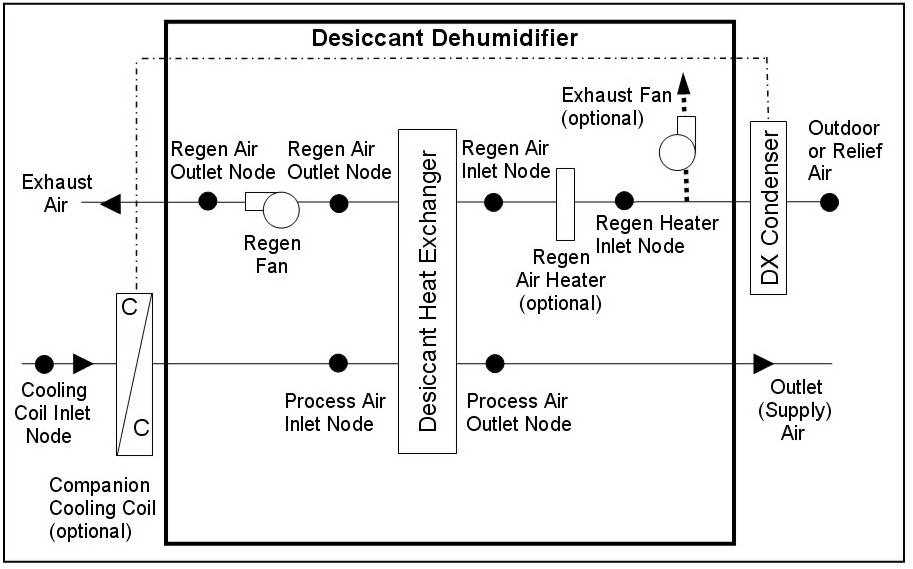
\includegraphics[width=0.9\textwidth, height=0.9\textheight, keepaspectratio=true]{media/image409.png}
\caption{Schematic of Dehumidifier:Desiccant:System with Draw Through Regeneration Fan Placement \protect \label{fig:schematic-of-dehumidifier-desiccant-system}}
\end{figure}

A schematic of the compound object Dehumidifier:Desiccant:Systemis shown in Figure~\ref{fig:schematic-of-dehumidifier-desiccant-system} with the draw through regeneration air fan placement. Figure~\ref{fig:schematic-of-dehumidifier-desiccant-system-001} shows the Dehumidifier:Desiccant:System object configured with the blow through regeneration air fan placement.

NOTE: As with any air loop compound object, the Dehumidifier:Desiccant:System object itself is specified on the \hyperref[airloophvac]{AirLoopHVAC} Branch or in the \hyperref[airloophvacoutdoorairsystemequipmentlist]{AirLoopHVAC:OutdoorAirSystem:EquipmentList} for an \hyperref[airloophvacoutdoorairsystem]{AirLoopHVAC:OutdoorAirSystem}. The children objects (e.g., desiccant heat exchanger, regeneration air fan, and optional regeneration air heater) must be specified separately in the input data file and their inlet/outlet connections must be as shown in Figure~\ref{fig:schematic-of-dehumidifier-desiccant-system} or Figure~\ref{fig:schematic-of-dehumidifier-desiccant-system-001}.

\begin{figure}[hbtp] % fig 142
\centering
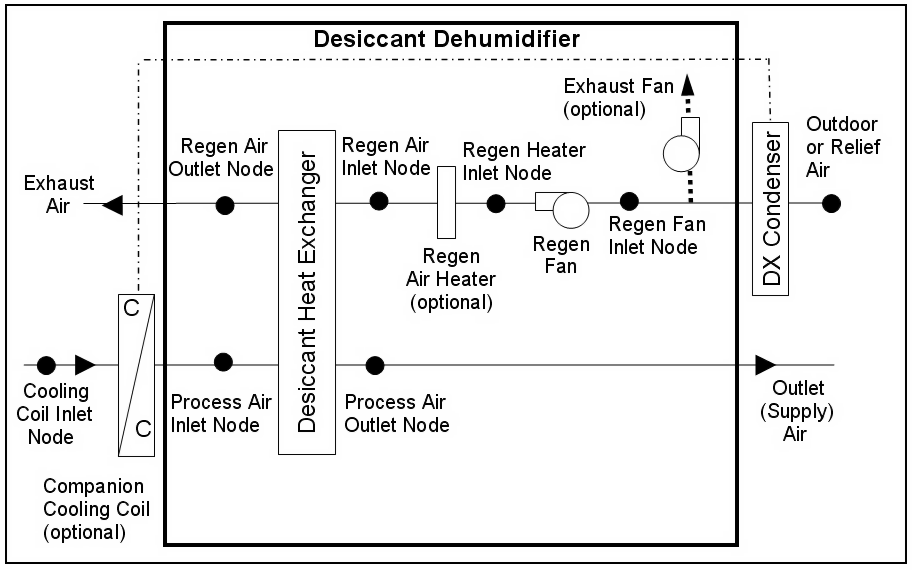
\includegraphics[width=0.9\textwidth, height=0.9\textheight, keepaspectratio=true]{media/image410.png}
\caption{Schematic of Dehumidifier:Desiccant:System with Blow Through Regeneration Fan Placement \protect \label{fig:schematic-of-dehumidifier-desiccant-system-001}}
\end{figure}

Currently the only heat exchanger choice for this object is HeatExchanger:Desiccant: BalancedFlow. So to model a Dehumidifier:Desiccant:System located in an air loop, the input data file should include the following objects:

\begin{itemize}
\item
  Dehumidifier:Desiccant:System (in an air loop (\hyperref[airloophvac]{AirLoopHVAC}) Branch or \hyperref[airloophvacoutdoorairsystemequipmentlist]{AirLoopHVAC:OutdoorAirSystem:EquipmentList} for an \hyperref[airloophvacoutdoorairsystem]{AirLoopHVAC:OutdoorAirSystem})
\item
  \hyperref[heatexchangerdesiccantbalancedflow]{HeatExchanger:Desiccant:BalancedFlow} (desiccant heat exchanger child object)
\item
  \hyperref[heatexchangerdesiccantbalancedflowperformancedatatype1]{HeatExchanger:Desiccant:BalancedFlow:PerformanceDataType1} (desiccant heat exchanger data object)
\item
  \hyperref[zonecontrolhumidistat]{ZoneControl:Humidistat}, and one of:
\item
  \hyperref[setpointmanagersinglezonehumiditymaximum]{SetpointManager:SingleZone:Humidity:Maximum}
\item
  \hyperref[setpointmanagermultizonehumiditymaximum]{SetpointManager:MultiZone:Humidity:Maximum}
\item
  \hyperref[setpointmanagermultizonemaximumhumidityaverage]{SetpointManager:MultiZone:MaximumHumidity:Average}
\item
  (when in an air loop (\hyperref[airloophvac]{AirLoopHVAC}) Branch), and \hyperref[setpointmanageroutdoorairpretreat]{SetpointManager:OutdoorAirPretreat} (when in an \hyperref[airloophvacoutdoorairsystem]{AirLoopHVAC:OutdoorAirSystem}) to place a maximum humidity ratio set point on the sensor node, typically the process air outlet node
\item
  \hyperref[fansystemmodel]{Fan:SystemModel}, \hyperref[fanonoff]{Fan:OnOff}, or \hyperref[fanconstantvolume]{Fan:ConstantVolume} (regeneration air fan)
\item
  \hyperref[coilheatingelectric]{Coil:Heating:Electric} or \hyperref[coilheatinggas-000]{Coil:Heating:Fuel} (optional regeneration air heater)
\item
  \hyperref[coilcoolingdxsinglespeed]{Coil:Cooling:DX:SingleSpeed}, \hyperref[coilcoolingdxvariablespeed]{Coil:Cooling:DX:VariableSpeed}, or \hyperref[coilcoolingdxtwostagewithhumiditycontrolmode]{Coil:Cooling:DX:TwoStageWithHumidityControlMode} (optional companion cooling coil)
\end{itemize}

If the user wants to model the Dehumidifier:Desiccant:System in an \hyperref[airloophvacoutdoorairsystem]{AirLoopHVAC:OutdoorAirSystem}, then the process air path of the dehumidifier should be located in the outdoor air stream and the regeneration air path may be placed in the relief air stream or modeled by the desiccant dehumidifier itself where the first node for the regeneration inlet air stream must be an outdoor air node. If the user wants to model the Dehumidifier:Desiccant:System in an air loop (\hyperref[airloophvac]{AirLoopHVAC}) Branch, then the process air path of the dehumidifier should be located in the air loop Branch object. For this case, the regeneration air stream is modeled by the desiccant dehumidifier object itself (i.e., not part of an air loop Branch statement) and the first node for the regeneration inlet air stream must be an outdoor air node (ref. Figure~\ref{fig:schematic-of-dehumidifier-desiccant-system} or Figure~\ref{fig:schematic-of-dehumidifier-desiccant-system-001}).

A description of each input field for this object is provided below:

\subsubsection{Inputs}\label{inputs-1-010}

\paragraph{Field: Name}\label{field-name-1-009}

A unique, user-assigned name for a particular Dehumidifier:Desiccant:System. Any reference to this dehumidifier by another object will use this name.

\paragraph{Field: Availability Schedule Name}\label{field-availability-schedule-name-1-002}

The name of the schedule (ref: Schedule) that denotes whether the dehumidifier can operate during a given time period. A schedule value greater than 0 (usually 1 is used) indicates that the dehumidifier can operate. A value less than or equal to 0 (usually 0 is used) denotes that the dehumidifier will not operate (i.e., no heat exchange will take place and the regeneration air fan does not operate). If the field is blank, the schedule has a value of 1 for all time periods. For the case where companion cooling coil regeneration air heating has been specified, the desiccant dehumidifier's exhaust fan serves as the condenser air fan for the cooling coil system so this availability schedule will not disable exhaust fan operation.

\paragraph{Field: Desiccant Heat Exchanger Object Type}\label{field-desiccant-heat-exchanger-object-type}

This alpha field contains the type of desiccant heat exchanger used with this dehumidifier. Currently, the only valid choice is \hyperref[heatexchangerdesiccantbalancedflow]{HeatExchanger:Desiccant:BalancedFlow}.

\paragraph{Field: Desiccant Heat Exchanger Name}\label{field-desiccant-heat-exchanger-name}

This alpha field contains the name of the desiccant heat exchanger used with this dehumidifier.

\paragraph{Field: Sensor Node Name}\label{field-sensor-node-name-000}

This alpha field specifies the name of the air loop node used to control desiccant heat exchanger operation. A set point manager must be used to place a maximum humidity ratio set point on this node (e.g., \hyperref[setpointmanagersinglezonehumiditymaximum]{SetpointManager:SingleZone:Humidity:Maximum} or \hyperref[setpointmanageroutdoorairpretreat]{SetpointManager:OutdoorAirPretreat}).

\paragraph{Field: Regeneration Air Fan Object Type}\label{field-regeneration-air-fan-object-type}

This alpha field contains the type of regeneration air fan used. Available fan types are \hyperref[fansystemmodel]{Fan:SystemModel}, \hyperref[fanonoff]{Fan:OnOff} and \hyperref[fanconstantvolume]{Fan:ConstantVolume}.

\paragraph{Field: Regeneration Air Fan Name}\label{field-regeneration-air-fan-name}

This alpha field contains the name of the regeneration air fan used with this dehumidifier.

\paragraph{Field: Regeneration Air Fan Placement}\label{field-regeneration-air-fan-placement}

This alpha field specifies the fan configuration used in the desiccant dehumidifier. Valid choices are BlowThrough and DrawThrough , with a default of DrawThrough if this field is left blank.

\paragraph{Field: Regeneration Air Heater Object Type}\label{field-regeneration-air-heater-object-type}

This alpha field contains the type of heating coil used to heat the regeneration air stream. This field may be left blank when no regeneration air heater is required. The hot water and steam heating coils require specifying plant loop, branches, and connector objects to support the heating coils, and are placed on the demand side of the plantloop. The hot water flow modulation through the regeneration air heating coil does not require additional controller or \hyperref[controllerwatercoil]{Controller:WaterCoil} object. The parent object (Dehumidifier:Desiccant:System) itself provides the ``controller'' function of modulating water flow. For autosizing regeneration air heating coil the \emph{Design Coil Inlet Air Condition} used is the outdoor air condition if the desiccant system is on the primary air loop, or else if the desiccant system is on outdoor air system then it is the return air condition. The \emph{Design Coil Outlet Air Temperature} is the \emph{Regeneration Inlet Air Setpoint Temperature} specified in the input field below. Valid heating coil choices are:

\begin{itemize}
\item
  \hyperref[coilheatingelectric]{Coil:Heating:Electric}
\item
  \hyperref[coilheatinggas-000]{Coil:Heating:Fuel}
\item
  \hyperref[coilheatingwater]{Coil:Heating:Water}
\item
  \hyperref[coilheatingsteam]{Coil:Heating:Steam}
\end{itemize}

\paragraph{Field: Regeneration Air Heater Name}\label{field-regeneration-air-heater-name}

This alpha field contains the name of the heating coil used to heat the regeneration air stream. This field may be left blank when no regeneration air heater is required.

\paragraph{Field: Regeneration Inlet Air Setpoint Temperature}\label{field-regeneration-inlet-air-setpoint-temperature}

This optional numeric field specifies the regeneration air inlet temperature setpoint in Celsius. The regeneration air heater and/or the companion coil regeneration air heating will be controlled to this temperature to the extent possible. This field may be left blank when no regeneration air heater is required or when control of the exhaust fan used with the companion coil regeneration air heating option is not required. If regeneration air heating coils is autosized, then the value of this input field is used as the \emph{Regeneration Air Heater Design Outlet Air Temperature} for the coil sizing calculation. The default value is 46.0 degrees.

\paragraph{Field: Companion Cooling Coil Object Type}\label{field-companion-cooling-coil-object-type}

This optional alpha field contains the type of companion cooling coil used with this desiccant dehumidifier. The only valid choices are \hyperref[coilcoolingdxsinglespeed]{Coil:Cooling:DX:SingleSpeed}, \hyperref[coilcoolingdxvariablespeed]{Coil:Cooling:DX:VariableSpeed}, and \hyperref[coilcoolingdxtwostagewithhumiditycontrolmode]{Coil:Cooling:DX:TwoStageWithHumidityControlMode}.

\paragraph{Field: Companion Cooling Coil Name}\label{field-companion-cooling-coil-name}

This optional alpha field contains the name of the companion cooling coil used with this desiccant dehumidifier. This field may be left blank when no companion cooling coil is being modeled.

\paragraph{Field: Companion Cooling Coil Upstream of Dehumidifier Process Inlet}\label{field-companion-cooling-coil-upstream-of-dehumidifier-process-inlet}

This choice field specifies if the companion cooling coil is located immediately upstream of the dehumidifiers process inlet. Valid choices are Yes and No. If Yes is selected, then the outlet air node for the companion cooling coil must be the same as the dehumidifier's process air inlet node (i.e., the process air inlet node name for the desiccant heat exchanger specified for this desiccant dehumidifier). For this case, the companion cooling coil and the desiccant dehumidifier are assumed to operate in tandem ; that is, if the simulation determines that the companion cooling coil is unable to meet the humidity set point specified on the sensor node based on its own operation, then the desiccant dehumidifier operates at the same time and for the same duration as the cooling coil to provide improved dehumidification. If No is selected, then the dehumidifier will control to the humidity set point specified on the sensor node to the extent possible. The default value is No if this field is left blank.

\paragraph{Field: Companion Coil Regeneration Air Heating}\label{field-companion-coil-regeneration-air-heating}

This choice field determines if the companion cooling coil's condenser waste heat is used to heat the regeneration inlet air. Valid choices are Yes and No. The default value is No if this field is left blank.

\paragraph{Field: Exhaust Fan Maximum Flow Rate}\label{field-exhaust-fan-maximum-flow-rate}

This optional numeric field contains the maximum fan volumetric flow rate for the exhaust fan in cubic meters per second. As noted previously, this exhaust fan is modeled internally by the Dehumidifier:Desiccant:System object and a separate fan object should NOT be specified in the input data file for this fan. This field is used only when a companion cooling coil is specified and the Companion Coil Regeneration Air Heating field is set to Yes . This field must be used in conjunction with the Exhaust Fan Maximum Power and the Exhaust Fan Power Curve Name input fields. The model assumes that the exhaust fan will operate as needed to maintain the Regeneration Inlet Air Setpoint Temperature , up to the maximum flow rate specified in this input field. If the desiccant dehumidifier is OFF for a simulation timestep but its companion cooling coil is operating and is specified to provide regeneration air heating, then the exhaust fan operates at this maximum air flow rate (i.e., this fan serves as the condenser fan for the companion cooling coil system when regeneration air heating is specified, so the inputs to the companion cooling coil object should not include the condenser fan energy since the condenser fan energy is modeled by the Dehumidifier:Desiccant:System object).

\paragraph{Field: Exhaust Fan Maximum Power}\label{field-exhaust-fan-maximum-power}

This optional numeric field contains the maximum power for the exhaust fan in Watts (i.e., at the Exhaust Fan Maximum Flow Rate). This field is used only when a companion cooling coil is used and the Companion Coil Regeneration Air Heating field is set to Yes . This field must be used in conjunction with the Exhaust Fan Maximum Flow Rate and the Exhaust Fan Power Curve Name input fields.

\paragraph{Field: Exhaust Fan Power Curve Name}\label{field-exhaust-fan-power-curve-name}

This optional alpha field contains the name of the exhaust fan power modifier curve. This field is used only when a companion cooling coil is used and the Companion Coil Regeneration Air Heating field is set to Yes . This field must be used in conjunction with the Exhaust Fan Maximum Flow Rate and the Exhaust Fan Maximum Power input fields. If this field is blank, the exhaust fan operates (when required) at the maximum power specified in the field above. The curve object type for this Exhaust Fan Power Curve Name must be \hyperref[curvecubic]{Curve:Cubic} or \hyperref[curvequadratic]{Curve:Quadratic}. The curve object (\hyperref[curvecubic]{Curve:Cubic} or \hyperref[curvequadratic]{Curve:Quadratic}) defines the change in exhaust fan power as a function of the ratio of the actual exhaust air flow rate divided by the maximum flow rate.

Following is an example input for this object:

\begin{lstlisting}

Dehumidifier:Desiccant:System,
  Desiccant 1,                         !- Name
  FanAvailSched,                     !- Availability Schedule Name
  HeatExchanger:Desiccant:BalancedFlow,   !- Desiccant Heat Exchanger Object Type
  Desiccant Heat Exchanger 1,   !- Desiccant Heat Exchanger Name
  HX Process Outlet Node,   !- Sensor Node Name
  Fan:SystemModel,           !- Regeneration Air Fan Object Type
  Desiccant Regen Fan,         !- Regeneration Air Fan Name
  DrawThrough,                         !- Regeneration Air Fan Placement
  Coil:Heating:Fuel,               !- Regeneration Air Heater Object Type
  Desiccant Regen Coil,       !- Regeneration Air Heater Name
  46.111111,                             !- Regeneration Inlet Air Setpoint Temperature {C}
  Coil:Cooling:DX:SingleSpeed,   !- Companion Cooling Coil Object Type
  Desiccant DXSystem Cooling Coil,   !- Companion Cooling Coil Name
  Yes,                           !- Companion Cooling Coil Upstream of Dehumidifier Process Inlet
  Yes,                                         !- Companion Coil Regeneration Air Heating
  1.05,                                       !- Exhaust Fan Maximum Flow Rate {m3/s}
  50,                                           !- Exhaust Fan Maximum Power {W}
  EXHAUSTFANPLF;                     !- Exhaust Fan Power Curve Name
\end{lstlisting}

\subsubsection{Outputs}\label{outputs-1-006}

\begin{itemize}
\item
  HVAC,Sum,Dehumidifier Removed Water Mass {[}kg{]}
\item
  HVAC,Average,Dehumidifier Removed Water Mass Flow Rate {[}kg/s{]}
\item
  HVAC,Average,Dehumidifier Part Load Ratio {[]}
\item
  HVAC,Average,Dehumidifier Exhaust Fan Electricity Rate {[}W{]}
\item
  HVAC,Sum,Dehumidifier Exhaust Fan Electricity Energy {[}J{]}
\end{itemize}

\paragraph{Dehumidifier Removed Water Mass {[}kg{]}}\label{dehumidifier-removed-water-mass-kg-1}

This output is the mass of water removed from the process air stream in kilograms for the timestep being reported.

\paragraph{Dehumidifier Removed Water Mass Flow Rate {[}kg/s{]}}\label{dehumidifier-removed-water-mass-flow-rate-kgs-1}

This output is the average rate of water removal from the process air stream in kilograms per second for the timestep being reported.

\paragraph{Dehumidifier Part Load Ratio {[]}}\label{dehumidifier-part-load-ratio-1}

This output is the fraction of time that the desiccant heat exchanger (and associated regeneration air heater and fans, if appropriate) operate for the timestep being reported.

\paragraph{Dehumidifier Exhaust Fan Electricity Rate {[}W{]}}\label{dehumidifier-exhaust-fan-electric-power-w}

This output is the average electric consumption rate for the exhaust fan in Watts for the timestep being reported.

\paragraph{Dehumidifier Exhaust Fan Electricity Energy {[}J{]}}\label{dehumidifier-exhaust-fan-electric-energy-j}

This output is the electric consumption for the exhaust fan in Joules for the timestep being reported. This output is also added to a meter with Resource Type = Electricity, EndUseKey = Cooling, GroupKey = System (ref. Output:Meter objects).